\chapter{Introduction}
\section{Background}
Flash systems are gaining their presence everywhere from mobile devices to servers with RAID and SAN architectures. SSD has become more popular due to their high speed, low noise, low power consumption and reliability. 

There are many reasons for flash storage picking up in the storage industry. 
\textbf{\textit{The main advantages of NAND flash are: }}
\begin{enumerate}

\item Better performance capabilities, speed in particular. Flash storage can get the system up and running in few seconds. Enterprises that need fast processing of their business applications and retrieve/store data quickly prefer flash storage systems. 

\item The durability is very high compared to hard drives which have mechanical parts like the spinning disks, head etc. The chances of losing data due to equipment mishandling is low. This feature is very important for the business who are more concerned about the security of their data. The absence of mechanical moving parts also contributes to higher performance. 

\item They consume very less power, thereby reducing the energy costs greatly.

\end{enumerate}
There are a few disadvantages of the flash system as well and \textbf{the main disadvantage which is of interest to us is the endurance.} 

\textbf{\textit{Endurance}} is just a fancy name for \textbf{\textit{life time}} of the storage systems. Endurance of a storage system is a very important aspect as it directly correlates to the lifetime of data. Compared to the hard drives, the NAND flash has a very low endurance. They have a finite program-erase cycles because of the process involved in the program erase operations for every write. \textbf{\textit{NAND flash uses two methodologies to write data: }} 
\begin{enumerate}

\item  Quantum Tunneling.
\item  Hot Electron Injection.
\end{enumerate}

Each write to these systems causes physical damage due to the above mechanisms. Refer figure \ref{fig:1} for quantum tunneling and refer figure \ref{fig:2} for hot electron injection method. The damages are due to the high heat generated. The oxide layer in the flash systems which are used to trap the charges is degraded every time a write is performed. The charge stored representing either a 0 or 1 cannot be differentiated due to the damage and hence the flash systems become unusable after this point. The damage eventually piles up to decrease the endurance time of the flash system. The other disadvantage of the flash systems compared to the hard drives is the cost per GB. NAND flash is much more expensive than the hard drives. The price of flash storage is gradually decreasing but currently SSD are more expensive.

\begin{figure}[h]
    \centering
    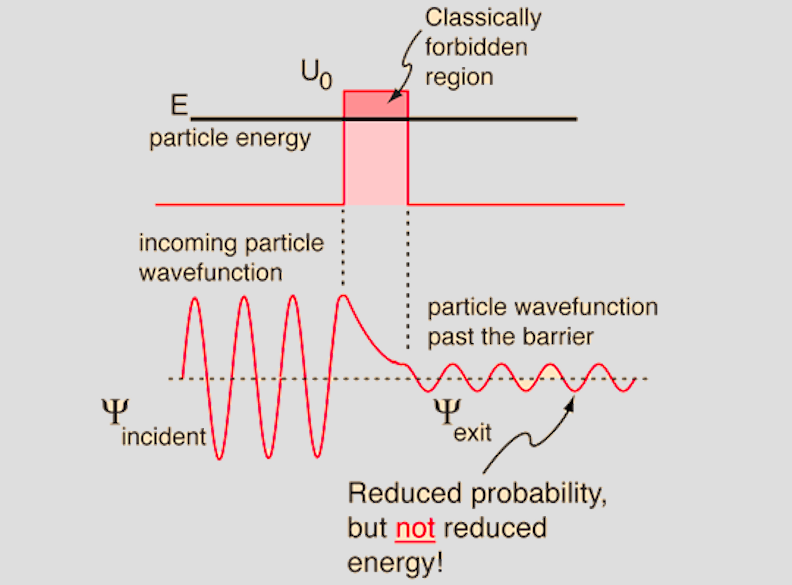
\includegraphics[width=\textwidth]{quantum}
    \caption{Quantum Tunneling \textsuperscript{[12]}}
    \label{fig:1}
\end{figure}

\begin{figure}[h]
    \centering
    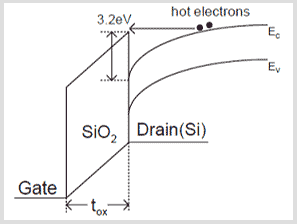
\includegraphics[width=\textwidth]{hot_electrons}
    \caption{Hot Electrons Injection\textsuperscript{[13]}}
    \label{fig:2}
\end{figure}
There are many distributed system applications which require a balance out between strong and eventual consistency. For example, consider an online shopping website. Use case such as the billing process should be strongly consistent whereas a recommendation window, based on the users` browsing history can be weakly consistent. For such systems, the proposed solution can be deployed for use cases which do not need strong consistency.

\section{Motivation}
When we consider the flash storage, we know that the number of writes which can be performed on flash storage is in the range of \textbf{$10^\textsuperscript{5}$ - $10^\textsuperscript{7}$}.
Due to the design of the flash memory, we cannot perform in-place update on a block of data. So we have to go through an erase of the block which completely erases the page by making all bits to zero (by having negative charge) and then perform the write cycle. But this leads to a condition called uneven wearing because a part of the storage is accessed rarely where the data is used only for reading (say a copy of the movie image) and the other part of the data is accessed often for writing (say a part of the disk which is used for paging). To solve this problem \textbf{“Wear Leveling”} was introduced.
 
 \textit{But wear leveling increases the number of writes in a flash storage} i.e. the \textbf{write amplification.}
 
 \textbf{\textit{The main idea of this research is to reduce the number of writes if the same piece of data is present in the RAM or in the storage replica which is about to change shortly.}}

\section{Development Environment}

The project was mainly developed in University of California Santa Cruz under the guidance of Professor Jishen Zhao in her lab. 

Initially it was proposed to develop the code in C language to support and run on Unix based Operating System running any data base. Later for simplicity and to increase the rate of development to implement the proof of concept it was decided to use Python language and pickel DB.

 Apart from the pickle DB package for this project we have used python packages like matplotlib, tox, socket and pytest which will be discussed in detail later.

For executing the program, we required minimum 2 separate computers to test the code.  Later moved to virtual environment by using the "Oracle virtual box" for dvelopment and test. The code has been tested on different operating systems like the MAC OS, Windows and Linux setup which were used both as a client and server configurations. More details about the architecture and system design is explanined later in the implementation section. 

%I have started the project from the scratch and uploaded my code under my git repository:  "https://github.com/Narendrakumarg1728/write_reduction_in_Distributed_replicas"

\textsuperscript{[1]} For the project we have used the python version 2.7. Install python version 2.7 by running the below commands on different Operating systems or can also be installed using Anaconda .


1. Ubuntu.

sudo apt-get install build-essential checkinstall
sudo apt-get install libreadline-gplv2-dev libncursesw5-dev libssl-dev libsqlite3-dev tk-dev libgdbm-dev libc6-dev libbz2-dev
cd ~/Downloads/
wget https://www.python.org/ftp/python/2.7.12/Python-2.7.12.tgz
tar -xvf Python-2.7.12.tgz
cd Python-2.7.12
./configure
make
sudo checkinstall

2. MAC OS.

Download package from "https://www.python.org/downloads/mac-osx/" then double click to install python.

3. Windows OS.

Download package from "https://www.python.org/downloads/windows/" then double click to install python. 


In order to test if the development environment is working as expected, type ``python -v". The versions of all the packages and the python version is displayed along with the python interpreter prompt at the end as shown in the figure \ref{fig:3}.

\begin{figure}[h]
    \centering
    \includegraphics[width=\textwidth]{python}
    \caption{Python version}
    \label{fig:3}
\end{figure}


\subsection{TOX}
Tox is a tool that creates a virtual environment for python. It is very helpful for creating a separate virtual environment for our development and testing.  Use the command "pip install tox" to install tox and then run the command "tox-quickstart" for setting up the environment as shown in the below figure \ref{fig:4}.

\begin{figure}[h]
    \centering
    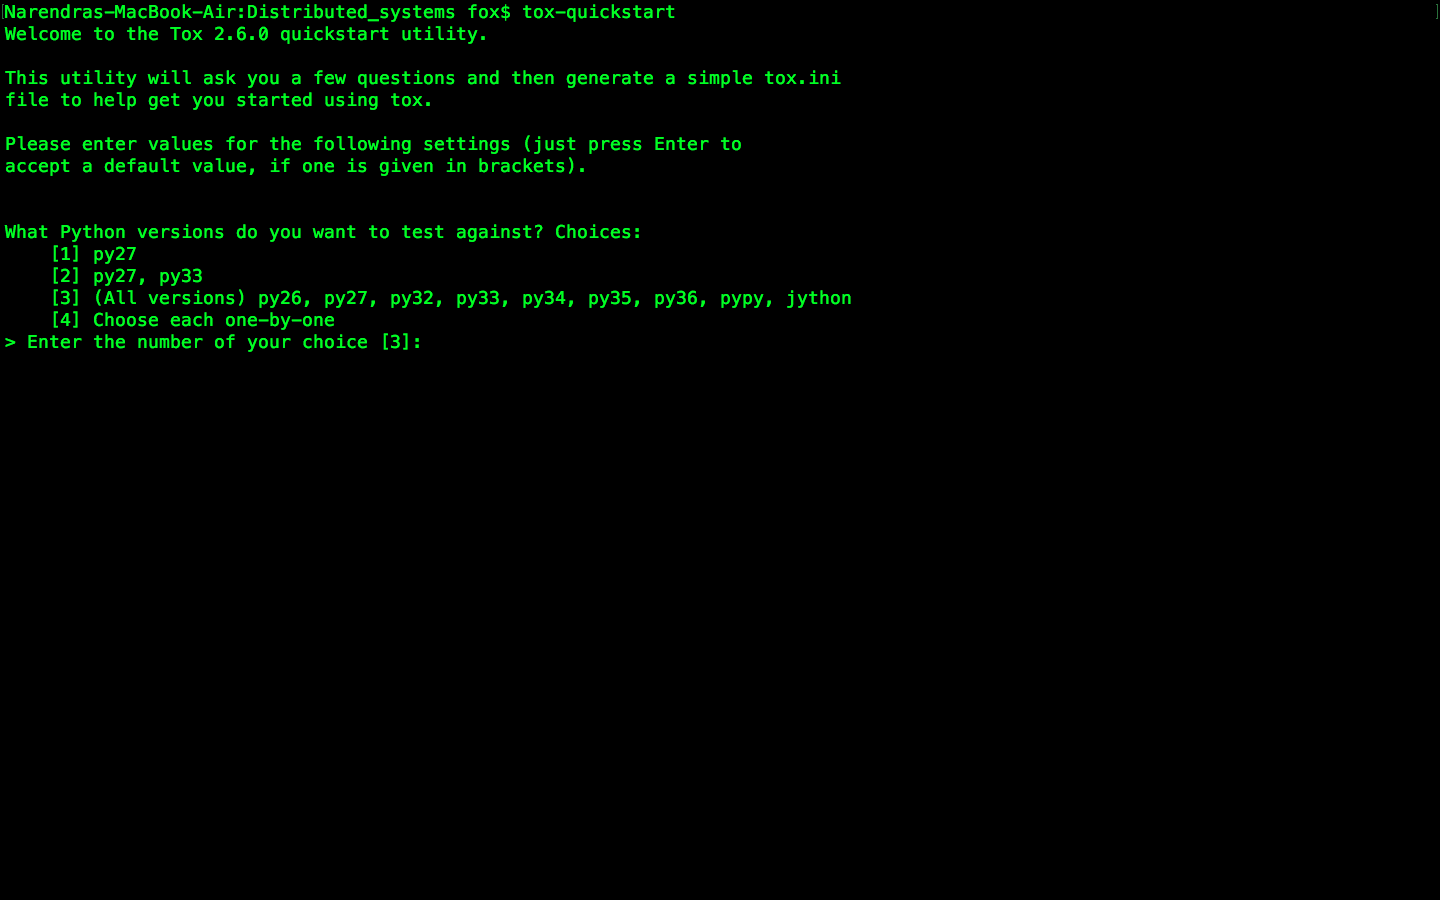
\includegraphics[width=\textwidth]{tox}
    \caption{tox-quickstart}
    \label{fig:4}
\end{figure}

\subsection{PYTEST}

For testing and debugging of the python code we have used the python test frame work pytest. To install pytest use the command "pip install pytest" then for debugging using pytest use the inbuilt function "assert" which will be discussed later in detail. To test and debug run the command pytest as shown in the figure \ref{fig:5}.

\begin{figure}[h]
    \centering
    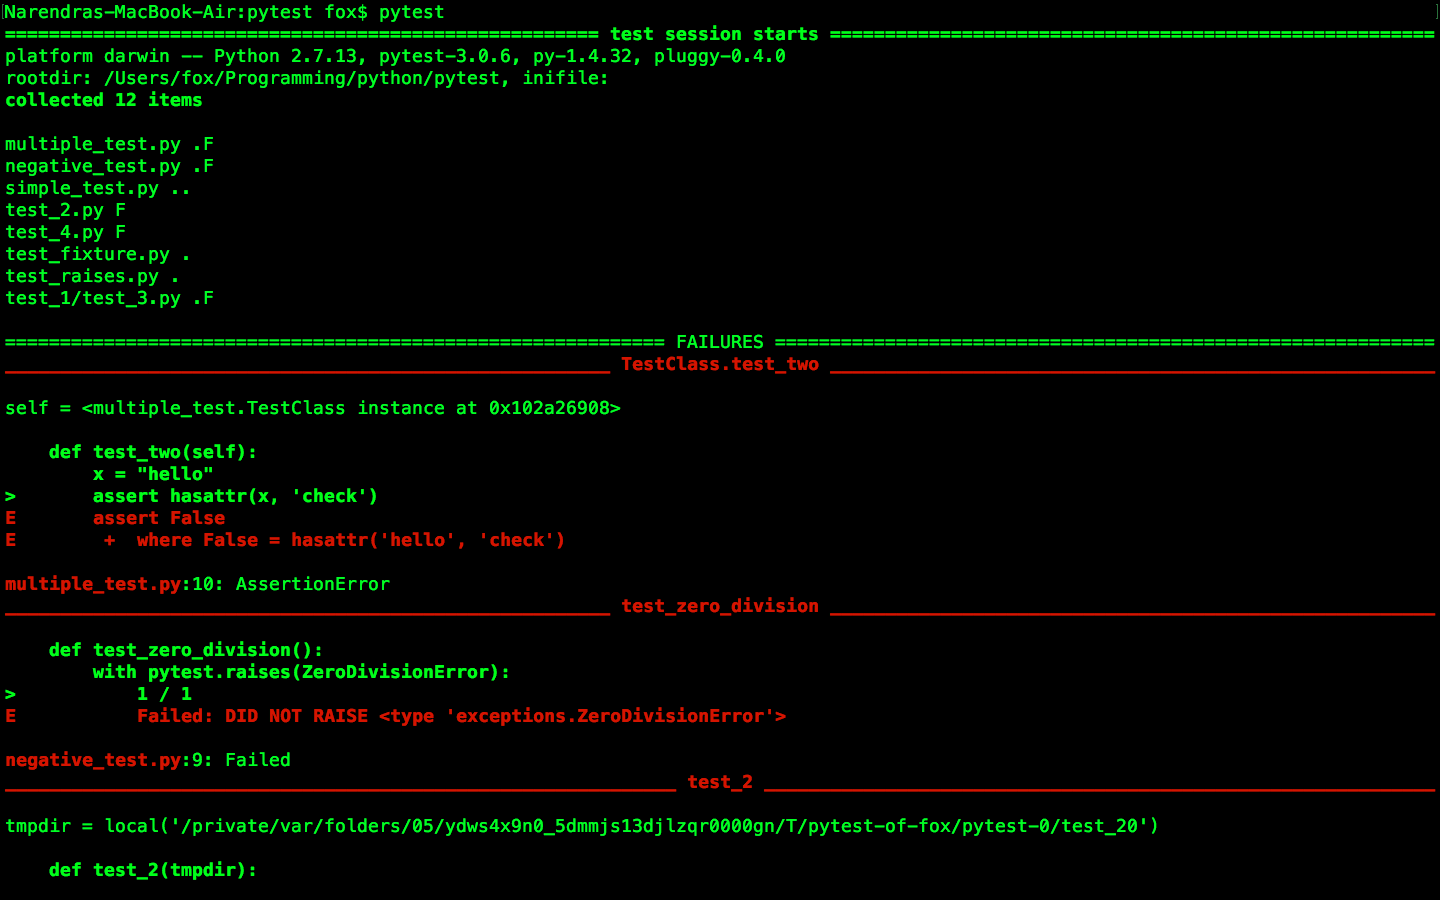
\includegraphics[width=\textwidth]{pytest}
    \caption{pytest for testing and debugging}
    \label{fig:5}
\end{figure}

\newpage
